\documentclass[]{article}
\usepackage{lmodern}
\usepackage{amssymb,amsmath}
\usepackage{ifxetex,ifluatex}
\usepackage{fixltx2e} % provides \textsubscript
\ifnum 0\ifxetex 1\fi\ifluatex 1\fi=0 % if pdftex
  \usepackage[T1]{fontenc}
  \usepackage[utf8]{inputenc}
\else % if luatex or xelatex
  \ifxetex
    \usepackage{mathspec}
    \usepackage{xltxtra,xunicode}
  \else
    \usepackage{fontspec}
  \fi
  \defaultfontfeatures{Mapping=tex-text,Scale=MatchLowercase}
  \newcommand{\euro}{€}
\fi
% use upquote if available, for straight quotes in verbatim environments
\IfFileExists{upquote.sty}{\usepackage{upquote}}{}
% use microtype if available
\IfFileExists{microtype.sty}{%
\usepackage{microtype}
\UseMicrotypeSet[protrusion]{basicmath} % disable protrusion for tt fonts
}{}
\usepackage[margin=1in]{geometry}
\usepackage{color}
\usepackage{fancyvrb}
\newcommand{\VerbBar}{|}
\newcommand{\VERB}{\Verb[commandchars=\\\{\}]}
\DefineVerbatimEnvironment{Highlighting}{Verbatim}{commandchars=\\\{\}}
% Add ',fontsize=\small' for more characters per line
\usepackage{framed}
\definecolor{shadecolor}{RGB}{248,248,248}
\newenvironment{Shaded}{\begin{snugshade}}{\end{snugshade}}
\newcommand{\KeywordTok}[1]{\textcolor[rgb]{0.13,0.29,0.53}{\textbf{{#1}}}}
\newcommand{\DataTypeTok}[1]{\textcolor[rgb]{0.13,0.29,0.53}{{#1}}}
\newcommand{\DecValTok}[1]{\textcolor[rgb]{0.00,0.00,0.81}{{#1}}}
\newcommand{\BaseNTok}[1]{\textcolor[rgb]{0.00,0.00,0.81}{{#1}}}
\newcommand{\FloatTok}[1]{\textcolor[rgb]{0.00,0.00,0.81}{{#1}}}
\newcommand{\CharTok}[1]{\textcolor[rgb]{0.31,0.60,0.02}{{#1}}}
\newcommand{\StringTok}[1]{\textcolor[rgb]{0.31,0.60,0.02}{{#1}}}
\newcommand{\CommentTok}[1]{\textcolor[rgb]{0.56,0.35,0.01}{\textit{{#1}}}}
\newcommand{\OtherTok}[1]{\textcolor[rgb]{0.56,0.35,0.01}{{#1}}}
\newcommand{\AlertTok}[1]{\textcolor[rgb]{0.94,0.16,0.16}{{#1}}}
\newcommand{\FunctionTok}[1]{\textcolor[rgb]{0.00,0.00,0.00}{{#1}}}
\newcommand{\RegionMarkerTok}[1]{{#1}}
\newcommand{\ErrorTok}[1]{\textbf{{#1}}}
\newcommand{\NormalTok}[1]{{#1}}
\usepackage{graphicx}
\makeatletter
\def\maxwidth{\ifdim\Gin@nat@width>\linewidth\linewidth\else\Gin@nat@width\fi}
\def\maxheight{\ifdim\Gin@nat@height>\textheight\textheight\else\Gin@nat@height\fi}
\makeatother
% Scale images if necessary, so that they will not overflow the page
% margins by default, and it is still possible to overwrite the defaults
% using explicit options in \includegraphics[width, height, ...]{}
\setkeys{Gin}{width=\maxwidth,height=\maxheight,keepaspectratio}
\ifxetex
  \usepackage[setpagesize=false, % page size defined by xetex
              unicode=false, % unicode breaks when used with xetex
              xetex]{hyperref}
\else
  \usepackage[unicode=true]{hyperref}
\fi
\hypersetup{breaklinks=true,
            bookmarks=true,
            pdfauthor={Abbas Rizvi},
            pdftitle={STA 546 - Homework 3},
            colorlinks=true,
            citecolor=blue,
            urlcolor=blue,
            linkcolor=magenta,
            pdfborder={0 0 0}}
\urlstyle{same}  % don't use monospace font for urls
\setlength{\parindent}{0pt}
\setlength{\parskip}{6pt plus 2pt minus 1pt}
\setlength{\emergencystretch}{3em}  % prevent overfull lines
\setcounter{secnumdepth}{0}

%%% Use protect on footnotes to avoid problems with footnotes in titles
\let\rmarkdownfootnote\footnote%
\def\footnote{\protect\rmarkdownfootnote}

%%% Change title format to be more compact
\usepackage{titling}

% Create subtitle command for use in maketitle
\newcommand{\subtitle}[1]{
  \posttitle{
    \begin{center}\large#1\end{center}
    }
}

\setlength{\droptitle}{-2em}
  \title{STA 546 - Homework 3}
  \pretitle{\vspace{\droptitle}\centering\huge}
  \posttitle{\par}
  \author{Abbas Rizvi}
  \preauthor{\centering\large\emph}
  \postauthor{\par}
  \predate{\centering\large\emph}
  \postdate{\par}
  \date{April 8, 2016}



\begin{document}

\maketitle


\section{Problem 1}\label{problem-1}

The data sets ``Les Miserables'' and ``Dolphins'' networks were accessed
from the Nexus repository using the \texttt{igraph::nexus.get} function
in \texttt{R}.

\begin{Shaded}
\begin{Highlighting}[]
\KeywordTok{library}\NormalTok{(igraph)}
\NormalTok{dolphins <-}\StringTok{ }\KeywordTok{nexus.get}\NormalTok{(}\StringTok{"dolphins"}\NormalTok{)}
\NormalTok{miserables <-}\StringTok{ }\KeywordTok{nexus.get}\NormalTok{(}\StringTok{"miserables"}\NormalTok{)}
\end{Highlighting}
\end{Shaded}

\texttt{dolphins} is an \texttt{igraph} object containing a dataset
pertianing to an undirected social network of frequent associations
between 62 dolphins in a community living off Doubtful Sound, New
Zealand. \texttt{miserables} is also an \texttt{igraph} object
containing a coappearance weighted network of characters in the French
novel \emph{Les Miserables} by Victor Hugo. Two characters are connected
if they appear in the same scene. The weight of the connection is the
number of common appearances.

Hierarchical random graphs (HRG) were used on \texttt{dolphins} and
\texttt{miserables} to perform the tasks subsequent subsections of
section 1.

\subsection{1.1 Reveal Communities and Construct MCMC-based
dendrogram}\label{reveal-communities-and-construct-mcmc-based-dendrogram}

\texttt{igraphdemo(\textquotesingle{}hrg\textquotesingle{})} was used as
a tutorial/guide for subsection 1.1. The same pipeline was used for both
the \texttt{dolphins} and \texttt{miserables} for this analysis.

The \texttt{dolphins} network was organized into a community structure
using the \texttt{igraph::optimal.community} function.
\texttt{optimal.community} calculates community structure of a graph by
maximizing the modulatrity measure over all possible partitions. The
communities for \texttt{dolphins} and \texttt{miserables} can be seen in
Figure 1 and 3, respectively. We can see the constructed communitie did
a good job identifying differing groups.

\begin{Shaded}
\begin{Highlighting}[]
\KeywordTok{load}\NormalTok{(}\StringTok{"dolphins_optcom.Rdata"}\NormalTok{) }\CommentTok{#optimal community}
\KeywordTok{V}\NormalTok{(dolphins)$comm <-}\StringTok{ }\KeywordTok{membership}\NormalTok{(dolphins.optcom) }\CommentTok{#membership gives vertices }
\KeywordTok{plot}\NormalTok{(dolphins.optcom, dolphins) }\CommentTok{#revelation of communities}
\end{Highlighting}
\end{Shaded}

\begin{figure}

{\centering 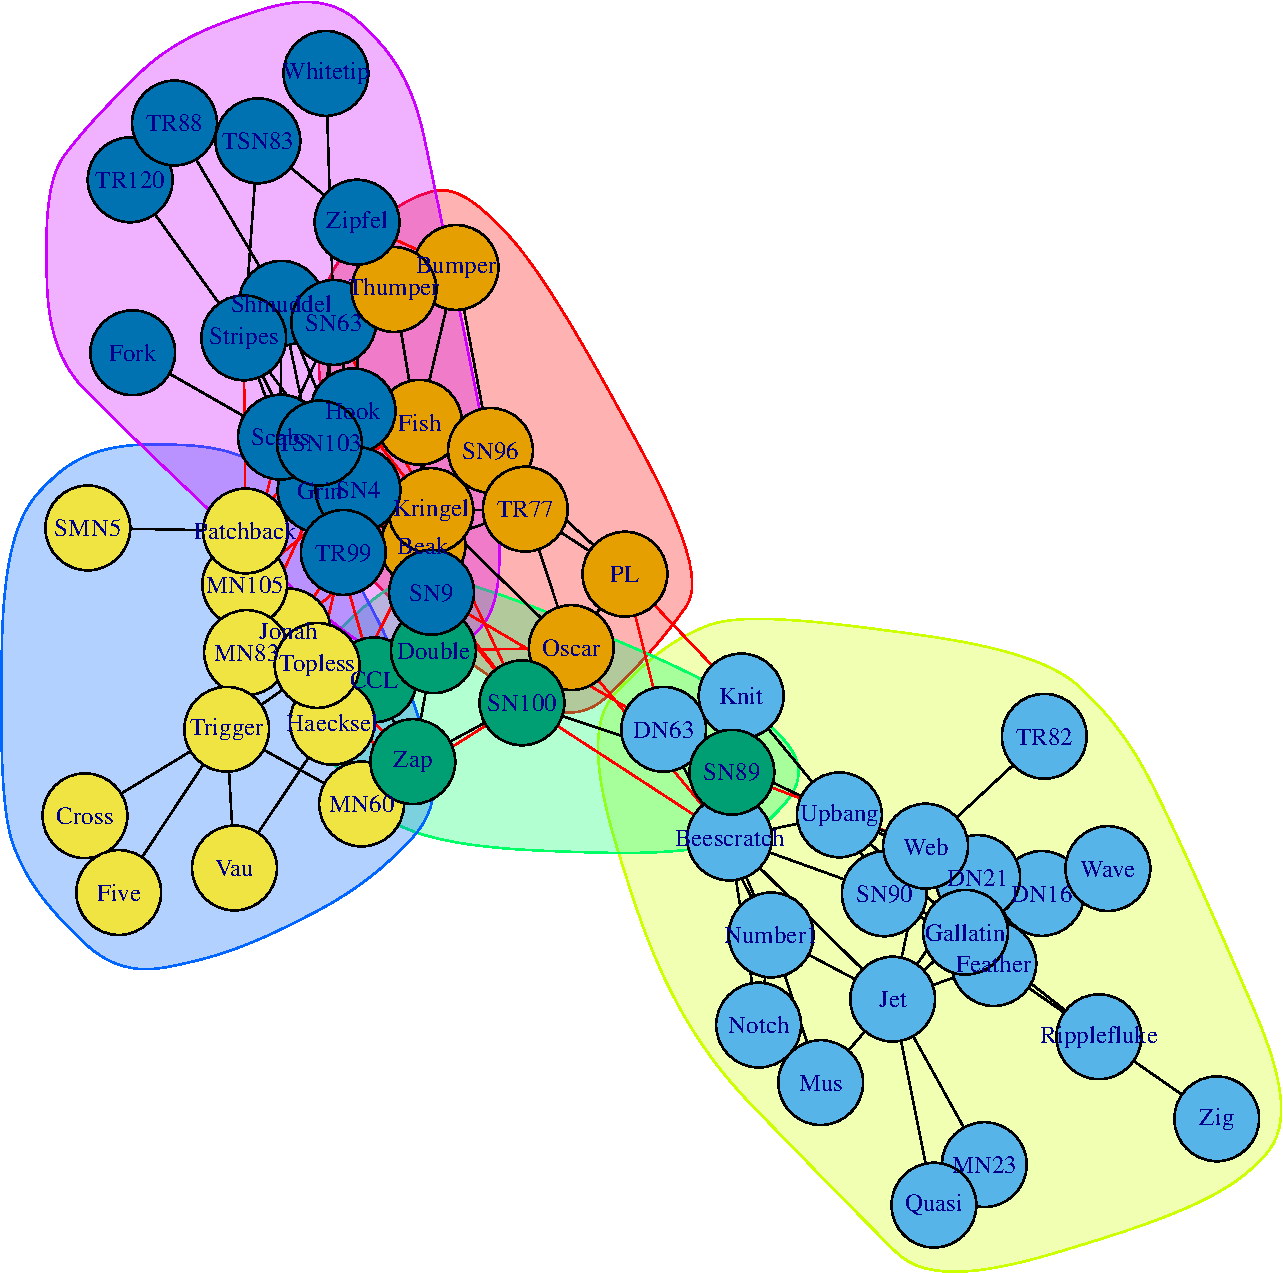
\includegraphics{sta546_hw3_files/figure-latex/unnamed-chunk-2-1} 

}

\caption{Clustered Dolphin Communities}\label{fig:unnamed-chunk-2}
\end{figure}

We now want to fit our \texttt{igraph} objects
(\texttt{dolphins}/\texttt{miserables}) to a HRG. HRG conducts MCMC
steps to perform the fitting until convergence. Dendrograms were
constructed using the \texttt{hrg} objects and we can see that for both
hrg-fitted \texttt{dolphin} and \texttt{miserables} datasets, that the
dendrograms were able to represent the clusters in a much cleaner
fashion than the community plots (Figure 2 and 4).

\begin{Shaded}
\begin{Highlighting}[]
\NormalTok{hrg <-}\StringTok{ }\KeywordTok{hrg.fit}\NormalTok{(dolphins) }\CommentTok{#MCMC sampling}
\KeywordTok{library}\NormalTok{(ape)}
\CommentTok{# plot it as dendrogram, looks better if the 'ape' package is installed}
\KeywordTok{plot_dendrogram}\NormalTok{(hrg, }\DataTypeTok{mode=}\StringTok{"phylo"}\NormalTok{, }\DataTypeTok{edge.color=}\StringTok{"black"}\NormalTok{, }\DataTypeTok{cex=}\FloatTok{0.8}\NormalTok{)}
\end{Highlighting}
\end{Shaded}

\begin{figure}

{\centering 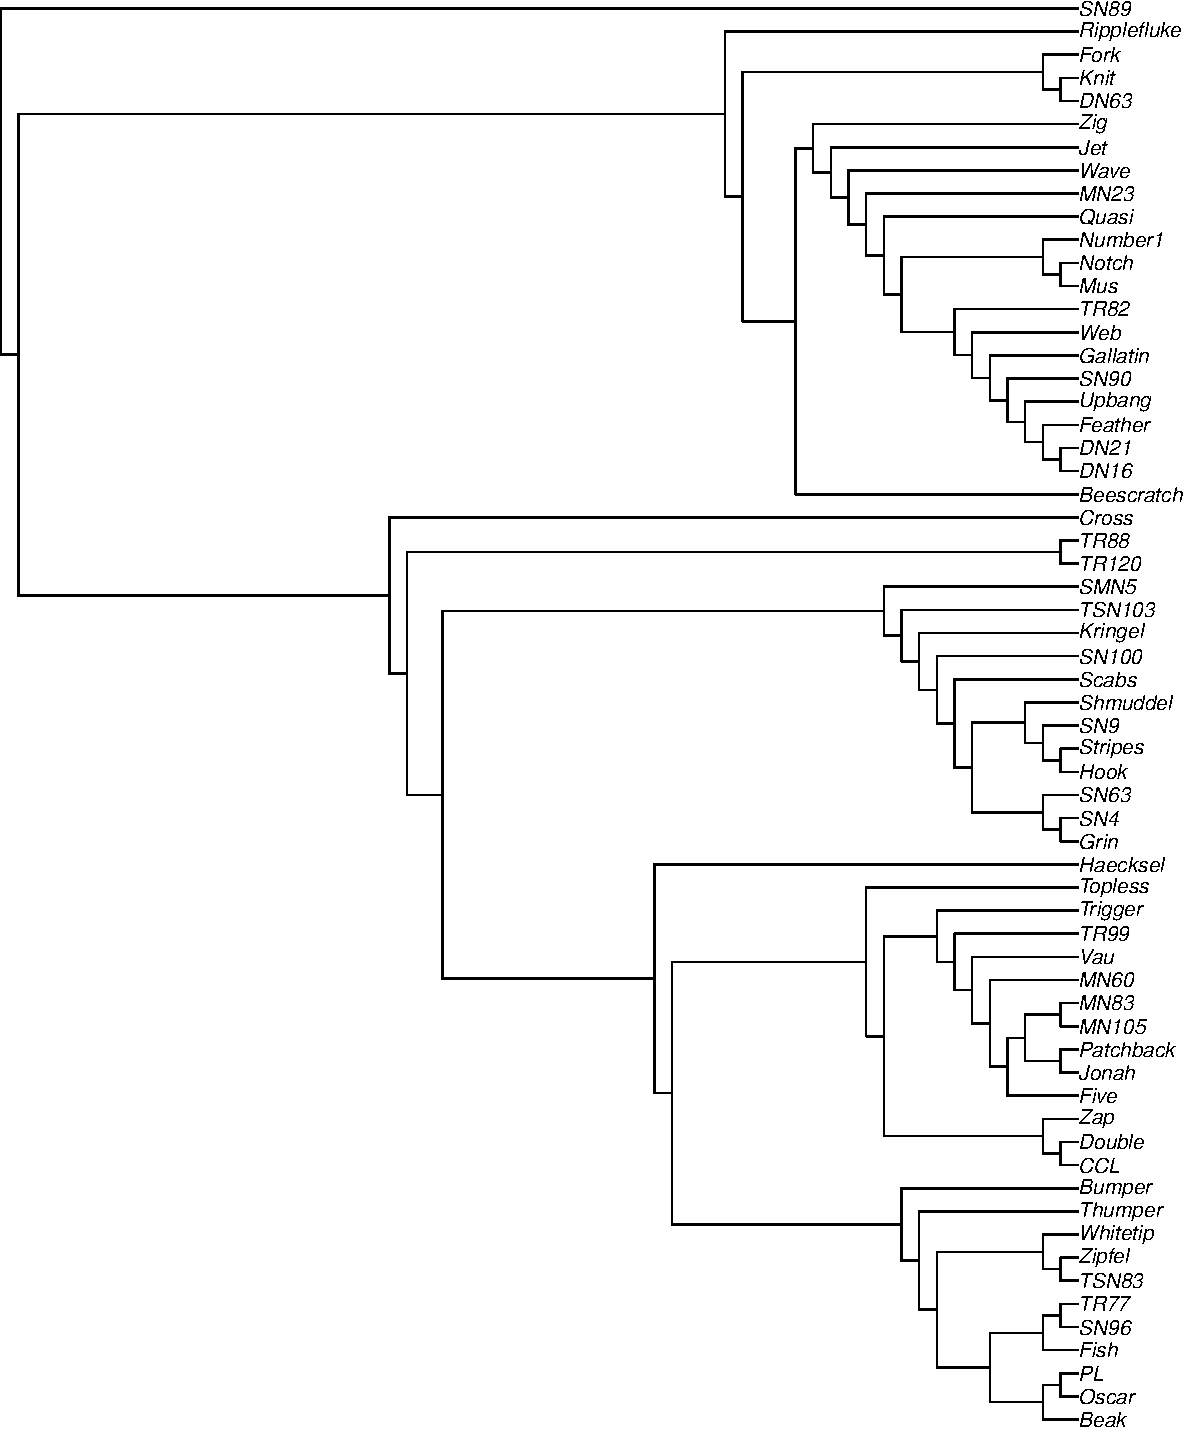
\includegraphics{sta546_hw3_files/figure-latex/unnamed-chunk-3-1} 

}

\caption{Dendrogram of MCMC-based Sampling of Dolphin Network}\label{fig:unnamed-chunk-3}
\end{figure}

\begin{figure}

{\centering 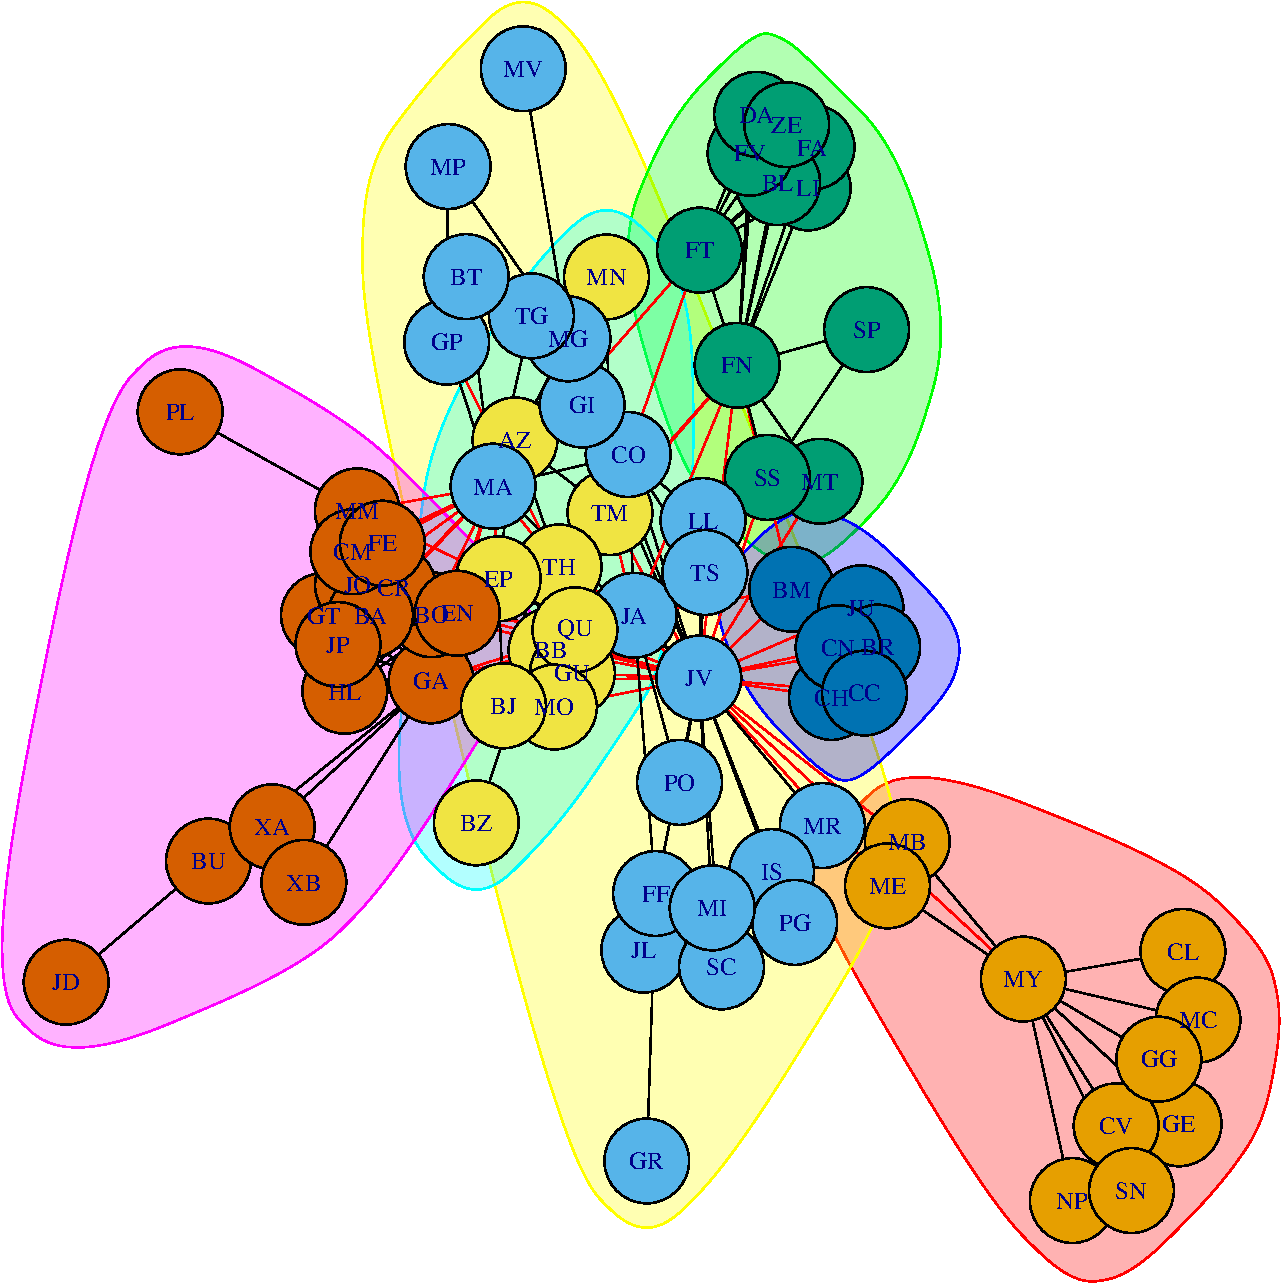
\includegraphics{sta546_hw3_files/figure-latex/unnamed-chunk-4-1} 

}

\caption{Clustered Les Miserables Communities}\label{fig:unnamed-chunk-4}
\end{figure}

\begin{figure}

{\centering 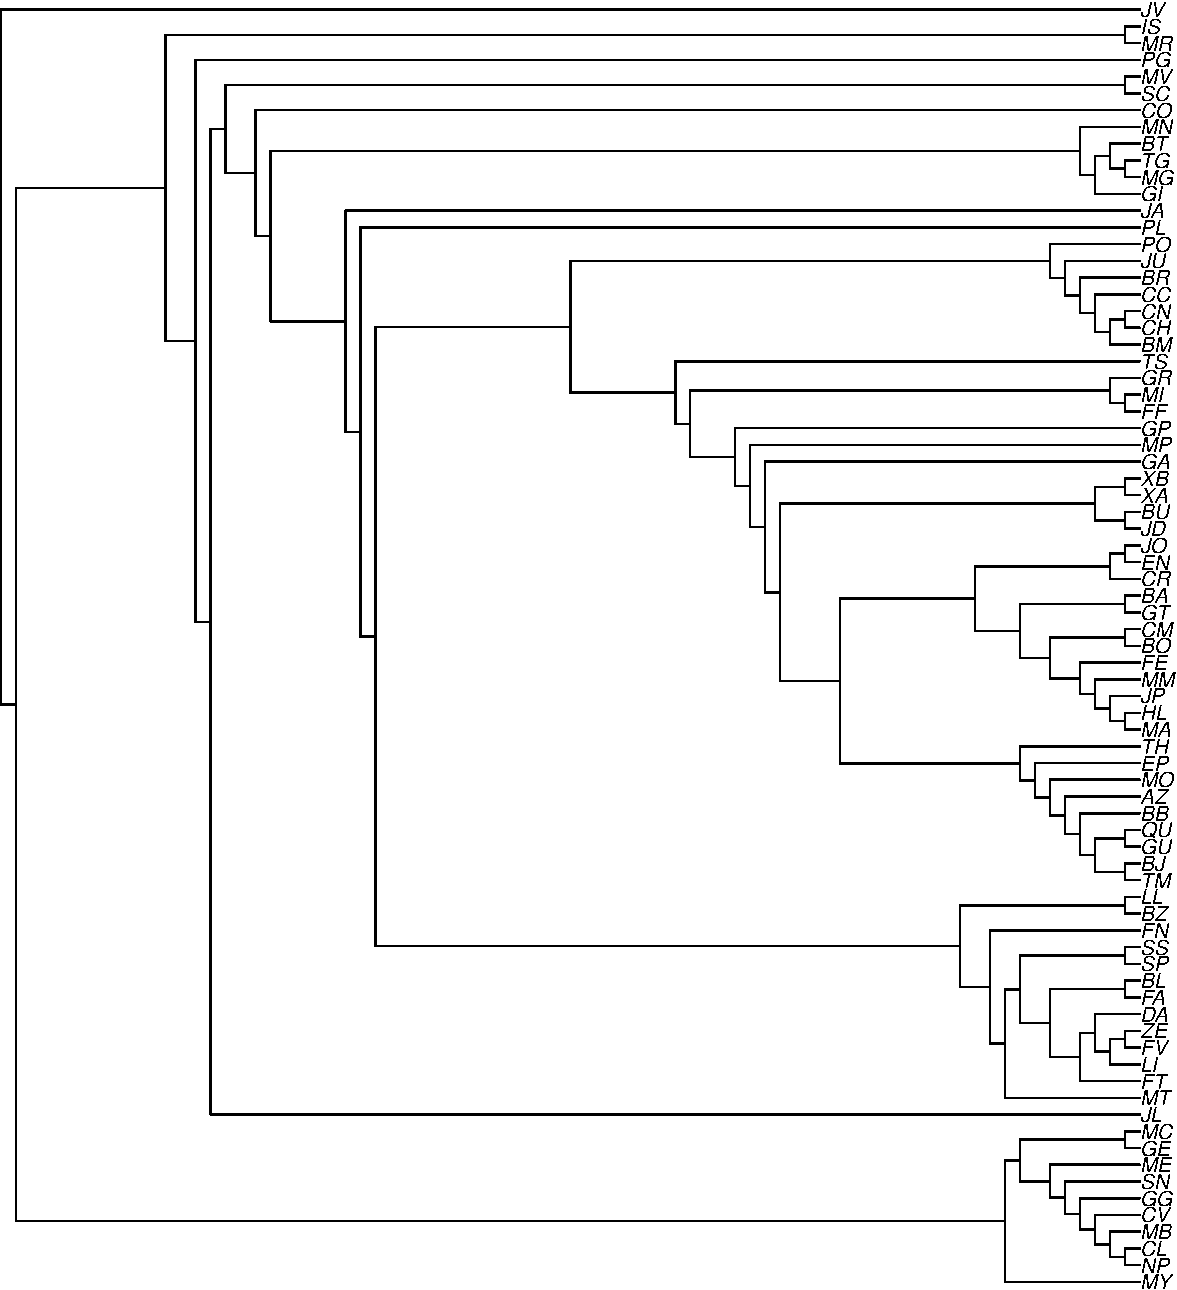
\includegraphics{sta546_hw3_files/figure-latex/unnamed-chunk-5-1} 

}

\caption{Dendrogram of MCMC-based Sampling of Les Miserables Network}\label{fig:unnamed-chunk-5}
\end{figure}

\subsection{1.2 Link-prediction of noisy versions of the Dolphin network
dataset}\label{link-prediction-of-noisy-versions-of-the-dolphin-network-dataset}

For section 1.2 we were asked to focus on the \texttt{dolphins} network
only. The helper function \texttt{link.prediction} was written such that
a user-specified percentage of random sampling of edges was conducted
and the sampled edges were subsequently deleted from the complete
datasets, with the purpose of creating a `noisy' dataset. We wanted to
see how well we were able to predict the edges that were deleted from
the complete dataset.

\begin{Shaded}
\begin{Highlighting}[]
\KeywordTok{set.seed}\NormalTok{(}\DecValTok{1}\NormalTok{)}
\KeywordTok{link.prediction}\NormalTok{(dolphins, }\DecValTok{5}\NormalTok{)}
\end{Highlighting}
\end{Shaded}

\begin{verbatim}
##      v1       v2        predicted probability
## [1,] "DN63"   "PL"      "0.0148"             
## [2,] "Double" "SN4"     "0.0768"             
## [3,] "Bumper" "Thumper" "0.0469"             
## [4,] "DN21"   "Web"     "0.299"              
## [5,] "DN63"   "Number1" "0.0511"             
## [6,] "DN16"   "Wave"    "0.0565"             
## [7,] "Jet"    "Web"     "0.3853"             
## [8,] "SN4"    "Topless" "0.0824"
\end{verbatim}

\texttt{link.prediction} was set to a 5 percent sampling deletion (8
edges of the 159) (See attached \texttt{R} code hw3.R for
\texttt{link.prediction}). The eight edges were able to be predicted by
\texttt{igraph::hrg.predict}. \texttt{igraph::hrg.predict} uses HRG
MCMC-sampling to predict missing edges from a network. This done using
the optimum model -- proportional to their likelihood. With the 5\%
deletion, the edges were predicted, but with low probabilities for the
most part, only two have \textgreater{}10\% probability of being
predicted.

\subsection{1.3 Repeating with 2.2 with more deletions (15\% and
40\%)}\label{repeating-with-2.2-with-more-deletions-15-and-40}

\begin{Shaded}
\begin{Highlighting}[]
\KeywordTok{link.prediction}\NormalTok{(dolphins, }\DecValTok{15}\NormalTok{)}
\end{Highlighting}
\end{Shaded}

\begin{verbatim}
##       v1           v2         predicted probability
##  [1,] "DN63"       "PL"       "0.015"              
##  [2,] "Double"     "SN4"      "0.0594"             
##  [3,] "Bumper"     "Thumper"  "0.0429"             
##  [4,] "DN21"       "Web"      "0.1553"             
##  [5,] "DN63"       "Number1"  "0.0492"             
##  [6,] "DN16"       "Wave"     "0.0571"             
##  [7,] "Jet"        "Web"      "0.3896"             
##  [8,] "SN4"        "Topless"  "0.0786"             
##  [9,] "Haecksel"   "Topless"  "0.1972"             
## [10,] "CCL"        "Grin"     "0.0465"             
## [11,] "Beescratch" "Number1"  "0.1182"             
## [12,] "Jonah"      "MN83"     "0.2065"             
## [13,] "Double"     "Zap"      "0.0816"             
## [14,] "Kringel"    "SN100"    "0.1076"             
## [15,] "Hook"       "TR99"     "0.089"              
## [16,] "DN63"       "SN9"      "0.003"              
## [17,] "Beak"       "TR77"     "0.1385"             
## [18,] "DN16"       "Web"      "0.1223"             
## [19,] "Scabs"      "Shmuddel" "0.2525"             
## [20,] "Shmuddel"   "TR88"     "0.0207"             
## [21,] "Stripes"    "TSN83"    "0.0248"             
## [22,] "Mus"        "Notch"    "0.1216"             
## [23,] "Bumper"     "Zipfel"   "0.0241"             
## [24,] "Beescratch" "Knit"     "0.08"
\end{verbatim}

\begin{Shaded}
\begin{Highlighting}[]
\KeywordTok{link.prediction}\NormalTok{(dolphins, }\DecValTok{40}\NormalTok{)}
\end{Highlighting}
\end{Shaded}

\begin{verbatim}
##       v1            v2            predicted probability
##  [1,] "DN63"        "PL"          "0.0256"             
##  [2,] "Double"      "SN4"         "0.0411"             
##  [3,] "Bumper"      "Thumper"     "0.0208"             
##  [4,] "DN21"        "Web"         "0.2015"             
##  [5,] "DN63"        "Number1"     "0.0256"             
##  [6,] "DN16"        "Wave"        "0.0055"             
##  [7,] "Jet"         "Web"         "0.2516"             
##  [8,] "SN4"         "Topless"     "0.0765"             
##  [9,] "Haecksel"    "Topless"     "0.0655"             
## [10,] "CCL"         "Grin"        "0.1153"             
## [11,] "Beescratch"  "Number1"     "0.033"              
## [12,] "Jonah"       "MN83"        "0.1388"             
## [13,] "Double"      "Zap"         "0.0813"             
## [14,] "Kringel"     "SN100"       "0.0595"             
## [15,] "Hook"        "TR99"        "0.0162"             
## [16,] "DN63"        "SN9"         "0.0064"             
## [17,] "Beak"        "TR77"        "0.0597"             
## [18,] "DN16"        "Web"         "0.1075"             
## [19,] "Scabs"       "Shmuddel"    "0.0261"             
## [20,] "Shmuddel"    "TR88"        "0.0125"             
## [21,] "Stripes"     "TSN83"       "0.0167"             
## [22,] "Mus"         "Notch"       "0.0794"             
## [23,] "Bumper"      "Zipfel"      "0.0189"             
## [24,] "Beescratch"  "Knit"        "0.0873"             
## [25,] "Double"      "Oscar"       "0.0284"             
## [26,] "MN105"       "Scabs"       "0.0243"             
## [27,] "DN16"        "Feather"     "0.0691"             
## [28,] "Hook"        "Scabs"       "0.0456"             
## [29,] "Scabs"       "TR99"        "0.028"              
## [30,] "Oscar"       "PL"          "0.1007"             
## [31,] "Scabs"       "SN4"         "0.0581"             
## [32,] "SN4"         "SN9"         "0.064"              
## [33,] "SN9"         "TSN103"      "0.0474"             
## [34,] "Jet"         "MN23"        "0.0211"             
## [35,] "Fish"        "TR77"        "0.0384"             
## [36,] "Fish"        "SN96"        "0.0621"             
## [37,] "MN60"        "Topless"     "0.1183"             
## [38,] "DN21"        "Jet"         "0.1658"             
## [39,] "SN4"         "Stripes"     "0.0556"             
## [40,] "Grin"        "Scabs"       "0.2628"             
## [41,] "Patchback"   "Trigger"     "0.2718"             
## [42,] "SN63"        "TSN103"      "0.0444"             
## [43,] "Shmuddel"    "Thumper"     "0.0163"             
## [44,] "SN100"       "SN4"         "0.0415"             
## [45,] "Hook"        "SN4"         "0.0517"             
## [46,] "Haecksel"    "Vau"         "0.0478"             
## [47,] "DN21"        "Feather"     "0.133"              
## [48,] "Ripplefluke" "Zig"         "0.0056"             
## [49,] "Bumper"      "SN96"        "0.0447"             
## [50,] "Five"        "Trigger"     "0.0068"             
## [51,] "Grin"        "Shmuddel"    "0.136"              
## [52,] "Double"      "Topless"     "0.0151"             
## [53,] "Feather"     "Ripplefluke" "0.0733"             
## [54,] "Haecksel"    "MN83"        "0.0616"             
## [55,] "Feather"     "Gallatin"    "0.3177"             
## [56,] "Beak"        "Haecksel"    "0.0646"             
## [57,] "Jet"         "Number1"     "0.0731"             
## [58,] "DN21"        "Wave"        "0.006"              
## [59,] "Hook"        "SN63"        "0.0455"             
## [60,] "MN105"       "Patchback"   "0.2599"             
## [61,] "Kringel"     "Thumper"     "0.1147"             
## [62,] "Beescratch"  "Notch"       "0.0234"             
## [63,] "SN100"       "Zap"         "0.0368"             
## [64,] "Topless"     "Zap"         "0.0207"
\end{verbatim}

\texttt{link.prediction} was used to randomly delete 15\% and 40\% of
the \texttt{dolphin} graph, respectively. It seems as the edges can
always be predicted regardless of the percent deletion, however, the
probability to be predicted remains relatively low for the most part,
but as sample deletion increases, there are more predicted values of
\textgreater{}10\% than in smaller deletions.

\section{Problem 2}\label{problem-2}

Exercise 3.11 from Koller et al. was adopted for this problem. The
following Bayesian Network (\texttt{B}) by Judea Pearl was considered:

\begin{figure}

{\centering 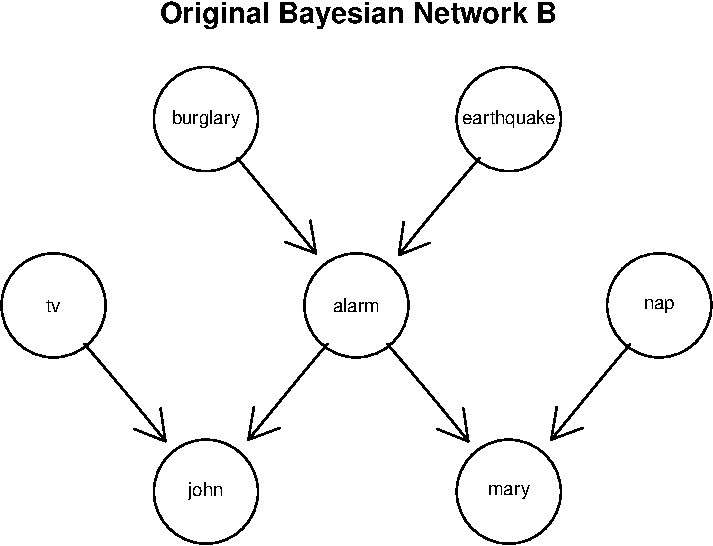
\includegraphics{sta546_hw3_files/figure-latex/unnamed-chunk-9-1} 

}

\caption{Original Bayesian Network B}\label{fig:unnamed-chunk-9}
\end{figure}

The original Bayesian Network \texttt{B} (Figure 5) was marginalized
over the \texttt{alarm} node. Subsequently, a Bayesian Network
\texttt{B\textquotesingle{}} was constructed such that it was the
minimal I-map for the marginal distribution
\(P_{B}(\text{B, E, T, N, J, M})\). The minimal I-map for the
marginalized network Bayesian Network \texttt{B\textquotesingle{}} was
constructed such that the independencies from \texttt{B} were preserved
(Figure 6) . We utilized the \texttt{ggm::inducedDAG} function in
\texttt{R} to construct this I-map.

\begin{figure}

{\centering 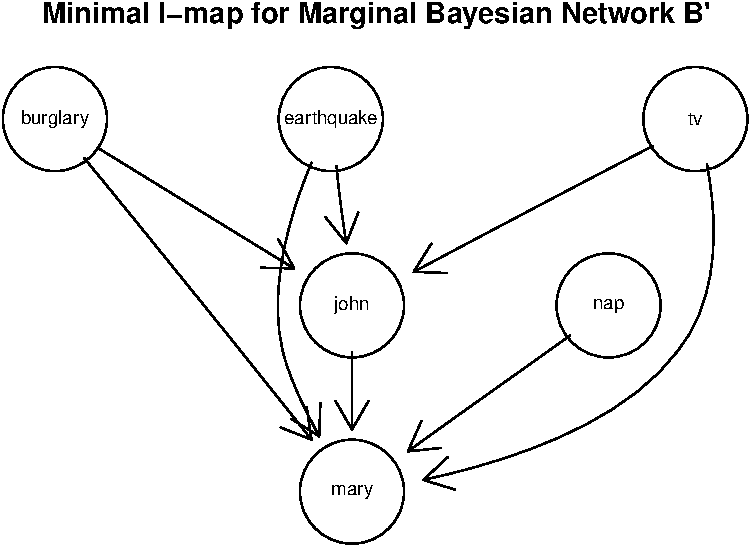
\includegraphics{sta546_hw3_files/figure-latex/unnamed-chunk-10-1} 

}

\caption{Bayesian Network B'}\label{fig:unnamed-chunk-10}
\end{figure}

\section{Problem 3}\label{problem-3}

A toy directed acyclic graph (DAG) was assembled in order to determine
d-separation between nodes (Figure 7).

\begin{figure}

{\centering 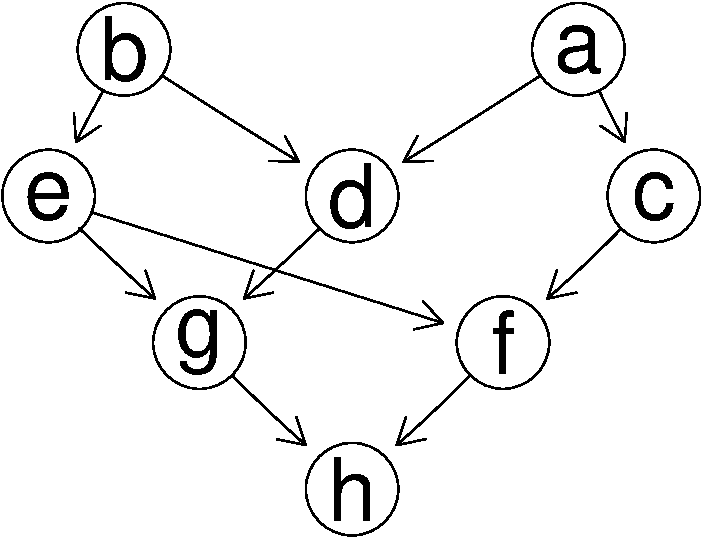
\includegraphics{sta546_hw3_files/figure-latex/unnamed-chunk-11-1} 

}

\caption{Toy DAG Model}\label{fig:unnamed-chunk-11}
\end{figure}

Determine if the following statements are ``\texttt{TRUE}'' or
``\texttt{FALSE}'' based on the DAG:

The helper function \texttt{dCon} was written for questions pertaining
to `d-connected' nodes

\begin{Shaded}
\begin{Highlighting}[]
\NormalTok{dCon <-}\StringTok{ }\NormalTok{function(dSep)\{}
        \NormalTok{if(dSep==}\OtherTok{FALSE}\NormalTok{)\{}
                \KeywordTok{as.logical}\NormalTok{(dSep}\DecValTok{+1}\NormalTok{)}
        \NormalTok{\}}
        \NormalTok{else\{}
                \KeywordTok{as.logical}\NormalTok{(dSep*}\DecValTok{0}\NormalTok{)}
        \NormalTok{\}}
\NormalTok{\}}
\end{Highlighting}
\end{Shaded}

\subsection{A) C and G are d-separated}\label{a-c-and-g-are-d-separated}

\begin{Shaded}
\begin{Highlighting}[]
\KeywordTok{dSep}\NormalTok{(}\KeywordTok{as}\NormalTok{(dag.list, }\StringTok{"matrix"}\NormalTok{), }\StringTok{"c"}\NormalTok{, }\StringTok{"g"}\NormalTok{, }\OtherTok{NULL}\NormalTok{)}
\end{Highlighting}
\end{Shaded}

\begin{verbatim}
## [1] FALSE
\end{verbatim}

\subsection{B) C and E are d-separated}\label{b-c-and-e-are-d-separated}

\begin{Shaded}
\begin{Highlighting}[]
\KeywordTok{dSep}\NormalTok{(}\KeywordTok{as}\NormalTok{(dag.list, }\StringTok{"matrix"}\NormalTok{), }\StringTok{"c"}\NormalTok{, }\StringTok{"e"}\NormalTok{, }\OtherTok{NULL}\NormalTok{)}
\end{Highlighting}
\end{Shaded}

\begin{verbatim}
## [1] TRUE
\end{verbatim}

\subsection{C) C and E are d-connected given evience about
G}\label{c-c-and-e-are-d-connected-given-evience-about-g}

\begin{Shaded}
\begin{Highlighting}[]
\KeywordTok{dCon}\NormalTok{(}\KeywordTok{dSep}\NormalTok{(}\KeywordTok{as}\NormalTok{(dag.list, }\StringTok{"matrix"}\NormalTok{), }\StringTok{"c"}\NormalTok{, }\StringTok{"e"}\NormalTok{, }\StringTok{"g"}\NormalTok{))}
\end{Highlighting}
\end{Shaded}

\begin{verbatim}
## [1] TRUE
\end{verbatim}

\subsection{D) A and G are d-connected given evidence about D and
E}\label{d-a-and-g-are-d-connected-given-evidence-about-d-and-e}

\begin{Shaded}
\begin{Highlighting}[]
\KeywordTok{dCon}\NormalTok{(}\KeywordTok{dSep}\NormalTok{(}\KeywordTok{as}\NormalTok{(dag.list, }\StringTok{"matrix"}\NormalTok{), }\StringTok{"a"}\NormalTok{, }\StringTok{"g"}\NormalTok{, }\KeywordTok{c}\NormalTok{(}\StringTok{"d"}\NormalTok{,}\StringTok{"e"}\NormalTok{)))}
\end{Highlighting}
\end{Shaded}

\begin{verbatim}
## [1] FALSE
\end{verbatim}

\subsection{E) A and G are d-connected given evidence on
D}\label{e-a-and-g-are-d-connected-given-evidence-on-d}

\begin{Shaded}
\begin{Highlighting}[]
\KeywordTok{dCon}\NormalTok{(}\KeywordTok{dSep}\NormalTok{(}\KeywordTok{as}\NormalTok{(dag.list, }\StringTok{"matrix"}\NormalTok{), }\StringTok{"a"}\NormalTok{, }\StringTok{"g"}\NormalTok{, }\StringTok{"d"}\NormalTok{))}
\end{Highlighting}
\end{Shaded}

\begin{verbatim}
## [1] TRUE
\end{verbatim}

\end{document}
